% draft.tex does not \input this file; kept because it holds material not copied into appendix.tex
\section{Stacking}
\label{sec:stacking}

We evaluate three pre-registered stack policies that combine each decision model with Amazon Bedrock Guardrails at strength medium.
Union blocks when either arm blocks.
Intersection blocks only when both block.
Cascade runs the decision model first and defers ambiguous scores between development-tuned cutoffs to the guardrail block bit, as summarized in Figure~\ref{fig:cascade}.
These stacks are distinct from the JailbreakBench post-hoc sensitivity stacks in Section~\ref{sec:jbb-sensitivity}; here the guardrail always uses the pre-registered crosswalk that maps harmful JailbreakBench labels to Prompt Attack only.
Stack metrics use the same tuned score thresholds and cascade cutoffs as the core pack.
Model and cascade thresholds were fit on the development pool under the medium-strength crosswalk guardrail bit.

We report stacks only on benchmarks where both arms supply a block decision and benign-known rows support false-positive rate (FPR).
Those evaluation sets are JailbreakBench ($n=200$, balanced harmful and benign splits), XSTest ($n=450$), and WildGuardMix ($n=1725$).
WildGuardMix FPR is computed on a small benign-known subset, so each additional benign false positive moves the rate by a large step; interpret WildGuardMix FPR cells with that granularity in mind.

Table~\ref{tab:stack-jbb} through Table~\ref{tab:stack-wgm} list miss rate and FPR for the decision model alone, guardrail alone, union, intersection, and cascade.
Guardrail-alone rows are identical across decision arms because they read the same cached Bedrock assessments.

\begin{table}[t]
  \centering
  \caption{Pre-registered stacks on JailbreakBench (guardrail strength medium).}
  \label{tab:stack-jbb}
  \begin{tabular}{llrr}
    \toprule
    Arm & Policy & Miss rate & FPR \\
    \midrule
    Jev & Model alone & 0.0300 & 0.3400 \\
    Jev & Guardrail alone & 0.9800 & 0.0000 \\
    Jev & Union & 0.0300 & 0.3400 \\
    Jev & Intersection & 0.9800 & 0.0000 \\
    Jev & Cascade & 0.0300 & 0.3400 \\
    \midrule
    Clef & Model alone & 0.0100 & 0.5400 \\
    Clef & Guardrail alone & 0.9800 & 0.0000 \\
    Clef & Union & 0.0100 & 0.5400 \\
    Clef & Intersection & 0.9800 & 0.0000 \\
    Clef & Cascade & 0.0100 & 0.5400 \\
    \midrule
    Clef-flash & Model alone & 0.0700 & 0.2400 \\
    Clef-flash & Guardrail alone & 0.9800 & 0.0000 \\
    Clef-flash & Union & 0.0700 & 0.2400 \\
    Clef-flash & Intersection & 0.9800 & 0.0000 \\
    Clef-flash & Cascade & 0.0700 & 0.2400 \\
    \bottomrule
  \end{tabular}
\end{table}

On JailbreakBench the pre-registered guardrail misses almost every harmful row (miss rate 0.9800, FPR 0.0000).
Union and cascade therefore match the decision model on miss and FPR for all three arms, because the model already blocks nearly all harmful prompts the guardrail would have caught.
Intersection matches the guardrail alone with miss rate 0.9800 and zero benign false positives.
Cascade cutoffs on JailbreakBench are $t_{\mathrm{high}}=t_{\mathrm{low}}=0.5$ for every arm, so deferral never engages and cascade coincides with the model path on this set.

\begin{table}[t]
  \centering
  \caption{Pre-registered stacks on XSTest (guardrail strength medium).}
  \label{tab:stack-xstest}
  \begin{tabular}{llrr}
    \toprule
    Arm & Policy & Miss rate & FPR \\
    \midrule
    Jev & Model alone & 0.1600 & 0.0120 \\
    Jev & Guardrail alone & 0.1700 & 0.0000 \\
    Jev & Union & 0.1000 & 0.0120 \\
    Jev & Intersection & 0.2300 & 0.0000 \\
    Jev & Cascade & 0.1250 & 0.0120 \\
    \midrule
    Clef & Model alone & 0.1050 & 0.1080 \\
    Clef & Guardrail alone & 0.1700 & 0.0000 \\
    Clef & Union & 0.0850 & 0.1080 \\
    Clef & Intersection & 0.1900 & 0.0000 \\
    Clef & Cascade & 0.0900 & 0.1080 \\
    \midrule
    Clef-flash & Model alone & 0.2400 & 0.0280 \\
    Clef-flash & Guardrail alone & 0.1700 & 0.0000 \\
    Clef-flash & Union & 0.1000 & 0.0280 \\
    Clef-flash & Intersection & 0.3100 & 0.0000 \\
    Clef-flash & Cascade & 0.1150 & 0.0280 \\
    \bottomrule
  \end{tabular}
\end{table}

XSTest is where stack choice moves the trade-off between harmful miss and benign false positives.
Union cuts miss relative to the decision model alone while leaving FPR unchanged for each arm (for example Jev miss falls from 0.1600 to 0.1000 at FPR 0.0120).
Intersection drives FPR to 0.0000 by requiring both arms to block, at the cost of higher miss than union (Jev intersection miss 0.2300 versus union 0.1000).
Cascade sits between model alone and union on miss for Jev and Clef-flash while preserving the model FPR.
Clef cascade miss 0.0900 is between its union value 0.0850 and model-alone 0.1050.

\begin{table}[t]
  \centering
  \caption{Pre-registered stacks on WildGuardMix (guardrail strength medium).}
  \label{tab:stack-wgm}
  \begin{tabular}{llrr}
    \toprule
    Arm & Policy & Miss rate & FPR \\
    \midrule
    Jev & Model alone & 0.6710 & 0.1923 \\
    Jev & Guardrail alone & 0.4208 & 0.4615 \\
    Jev & Union & 0.3661 & 0.5385 \\
    Jev & Intersection & 0.7257 & 0.1154 \\
    Jev & Cascade & 0.6710 & 0.1923 \\
    \midrule
    Clef & Model alone & 0.5750 & 0.5000 \\
    Clef & Guardrail alone & 0.4208 & 0.4615 \\
    Clef & Union & 0.3378 & 0.6923 \\
    Clef & Intersection & 0.6580 & 0.2692 \\
    Clef & Cascade & 0.5750 & 0.5000 \\
    \midrule
    Clef-flash & Model alone & 0.7334 & 0.0000 \\
    Clef-flash & Guardrail alone & 0.4208 & 0.4615 \\
    Clef-flash & Union & 0.3708 & 0.4615 \\
    Clef-flash & Intersection & 0.7834 & 0.0000 \\
    Clef-flash & Cascade & 0.7334 & 0.0000 \\
    \bottomrule
  \end{tabular}
\end{table}

WildGuardMix shows the largest stack-induced separation.
Union improves harmful miss versus both alone arms for Jev and Clef (Jev union miss 0.3661 versus model 0.6710 and guardrail 0.4208) but raises FPR sharply because either arm can flag benign prompts.
Intersection lowers FPR relative to union at higher miss (Jev intersection FPR 0.1154 versus union 0.5385).
For Jev, cascade equals model alone because tuned cutoffs $t_{\mathrm{high}}=0.78$ and $t_{\mathrm{low}}=0.77$ leave no score band that triggers guardrail deferral on this test set.
Clef-flash shows the same degeneracy: cascade and model alone both report miss 0.7334 and FPR 0.0000.

Figure~\ref{fig:miss-fpr} plots miss rate against FPR for core-pack arms and these stack points across datasets.
Together, the tables show that stack value depends on guardrail coverage on the benchmark.
Where the guardrail barely fires on harmful rows (JailbreakBench under the crosswalk), union and cascade cannot beat the model.
Where both arms disagree on harm and benign errors (WildGuardMix and XSTest), union and intersection trace distinct risk profiles.

\begin{figure}[t]
  \centering
  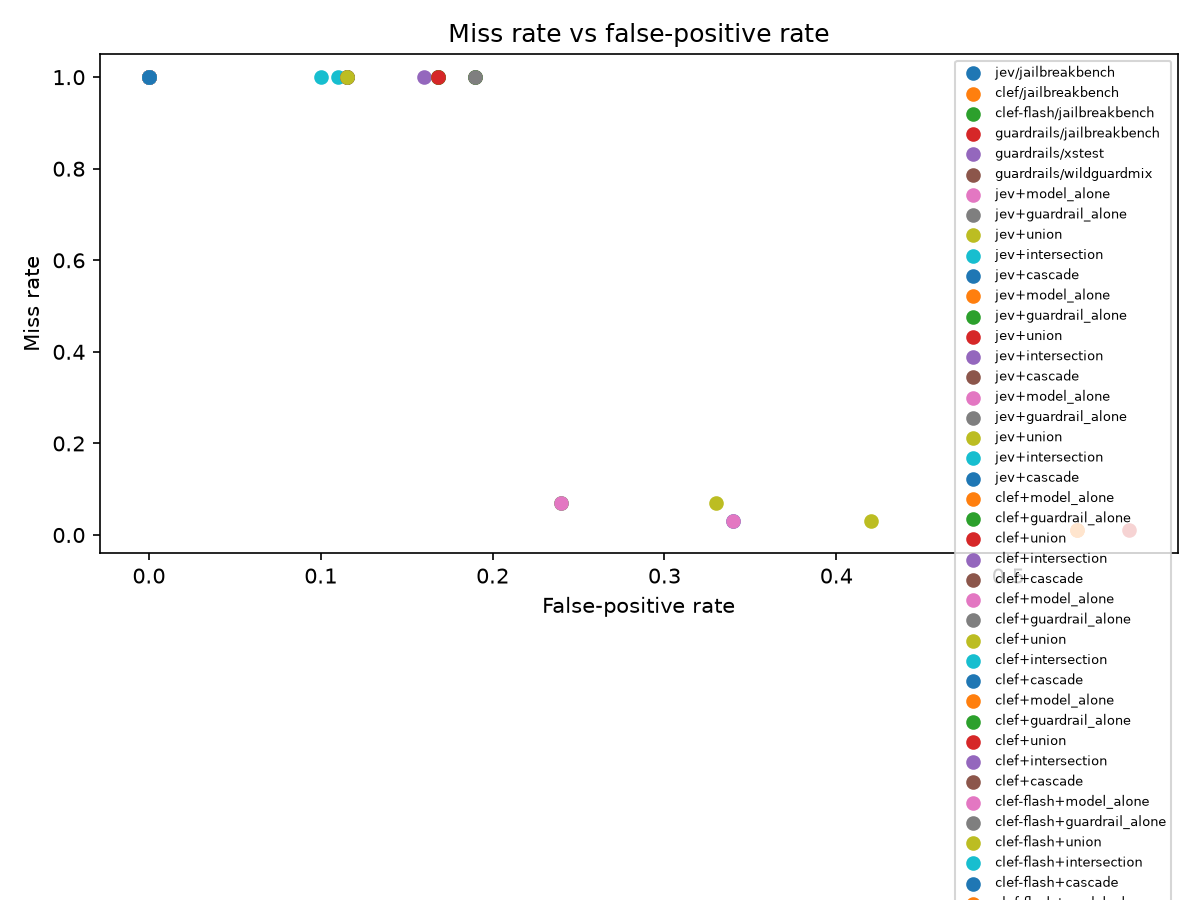
\includegraphics[width=\linewidth]{../outputs/figures/20261020T040920Z_90c5fd13/miss_vs_fpr.png}
  \caption{Miss rate versus false-positive rate for decision models, guardrails, and pre-registered stacks on JailbreakBench, XSTest, and WildGuardMix.}
  \label{fig:miss-fpr}
\end{figure}
